\documentclass[a4paper,12pt]{article}
\usepackage[utf8]{inputenc}
\usepackage[T2A]{fontenc}
\usepackage[russian,english]{babel}
\usepackage[pdftex]{graphics}
\DeclareGraphicsExtensions{.pdf,.png,.jpg}
\graphicspath{{pictures/}}
\begin{document}
\begin{center}
Санкт-Петербургский государственный политехнический университет
\\Кафедра компьютерных систем и программных технологий
\end{center}
\vspace*{10em plus .6em minus .5em}

\begin{center}
{\LARGEТелекоммуникационные технологии
\\Лабораторная работа №2
\\Ряд Фурье. Преобразование Фурье. Корреляция}
\end{center}

\vspace*{5em plus .6em minus .5em}
\begin{flushright}
Выполнил:\\студент гр.33501/4\\Курякин Д. А.\\Проверила:\\Богач Н.В.
\end{flushright}

\vspace*{15em plus .6em minus .5em}
\begin{center}
{\smallСанкт-Петербург
\\2018}
\end{center}
\pagestyle{empty}
\newpage
\pagestyle{plain}
\section{Цель работы}

Получить представление о спектрах телекоммуникационных сигналов.

\section{Постановка задачи}

\begin{itemize}
 \itemДля сигналов, построенных в лабораторной работе №1, вы-полните расчет преобразования Фурье. Перечислите свойства преобразования Фурье.

 \itemС помощью функции корреляции найдите позицию синхро-посылки [101] в сигнале [0001010111000010]. Получите пакет данных, если известно, что его длина составляет 8 бит без учета синхропосылки. Вычислите корреляцию прямым мето-дом, воспользуйтесь алгоритмом быстрой корреляции, сравни-те время работы обоих алгоритмов.

 \itemБыстрая корреляция
\end{itemize}

\section{Теоретический раздел}

\subsection{Свойства преобразования Фурье}
Основные свойства преобразования Фурье (ПФ):
\begin{enumerate}
	\item Линейность\\
    Преобразование Фурье относится к числу линейных интегральных операций, т.е. спектр суммы сигналов равен сумме спектров этих сигналов.
    \item Запаздывание\\
   Если происходит запаздывание (сдвиг, смещение) сигнала на $\tau$, то его спектральная функция умножается на $e^{-j\omega \tau}$ . Это приводит к изменению фазочастотной функции спектра (фазового угла всех гармоник) на величину - $-\omega \tau$ без изменения модуля (амплитудной функции) спектра.
    \item Изменения масштаба аргумента функции\\
   Изменение длительности сигнала в $a$ раз, где $a$ -- постоянный коэффициент, то ПФ с $Y(f)$ изменится на $\frac{1}{|a|}Y(\frac{f}{a})$.
    \item Дифференцирование функции\\
    Для получения спектра производной надо умножить исходный спектр на $j \omega$.
     \item Интегрирование функции\\
    При интегрировании от $-{\infty}$ до $t$ функции, имеющей равную нулю постоянную составляющую, ее ПФ делится на $j2{\pi}f$.
    \item Спектр произведения сигналов\\
    Спектр произведения сигналов представляет собой свертку их спектров, деленную на 2$\pi$.
    $F[x(t)y(t)]={\frac{1}{2{\pi}}}[X(f)*Y(f)]$
    \item Спектр свертки сигналов.\\
    ПФ свертки двух функций равно произведению ПФ свертываемых функции: $F[x(t)*y(t)]=X(f)Y(f)$
\end{enumerate}

\subsection{Корреляция}
Корреляция дает возможность установить в сигналах (или в рядах цифровых данных сигналов) наличие определенной связи изменения значений сигналов по независимой переменной, то есть, когда большие значения одного сигнала (относительно средних значений сигнала) связаны с большими значениями другого сигнала (положительная корреляция), или, наоборот, малые значения одного сигнала связаны с большими значениями другого (отрицательная корреляция), или данные двух сигналов никак не связаны (нулевая корреляция).
Дискретная кросс-корреляция функций $f(t)$ и $g(t)$:\\\\
$corr(f,g)[n] = {\sum_{m=-{\infty}}^{\infty}}f(m)g(n+m)$
, где $m$ -- величина задержки. \\\\
Чаще всего применяется кросс-корреляция в обработке сигналов, при этом $f$ считается образцом, а $g$ сигналом, содержащим образец.\\
 Результат -- это вектор чисел, показывающих, насколько сильно образец выражен в сигнале.\\
Чтобы ускорить расчёт используется теорема о корреляции, которая формулируется следующим образом:\\\\
$r_{12}(j)={\frac{1}{N}}F_D^{-1}[X(k)Y(k)]$
, где $F_D^{-1}$ это обратное дискретное преобразование Фурье.\\\\
Данный подход требует выполнения двух дискретных преобразований Фурье и одного обратного, что легче всего сделать, используя алгоритм БПФ. Если число членов в последовательностях достаточно велико, данный метод БПФ дает результат быстрее, чем непосредственный расчет взаимной корреляции. 
\newpage

\section{Ход работы}
\begin{enumerate}
{\itemИмеется синхропосылка [1 0 1] и сигнал [0 0 0 1 0 1 0 1 1 1 0 0 0 0 1 0]
\center{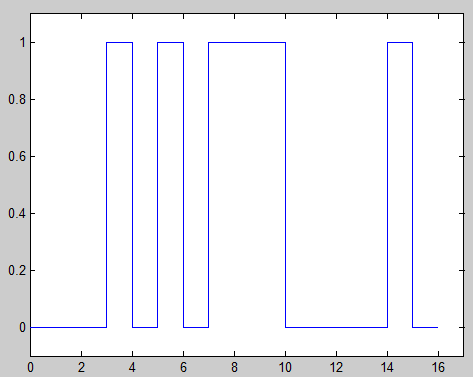
\includegraphics{./pictures/signal.png} \\ Рис.1 Сигнал}
\\}

{\itemДля нахождения позиции синхропосылки в сигнале воспользуемся алгоритмами кросс-корреляции и быстрой корреляции.
\center{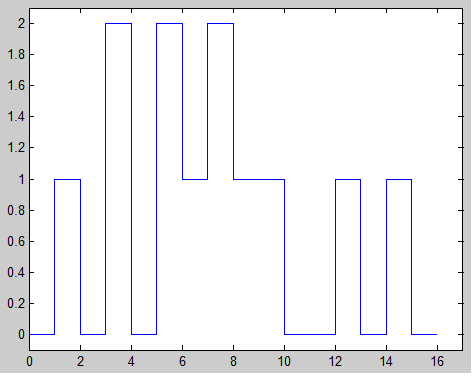
\includegraphics{./pictures/xcorr.png} \\ Рис.2 Результаты вычисления кросс-корреляции}
\center{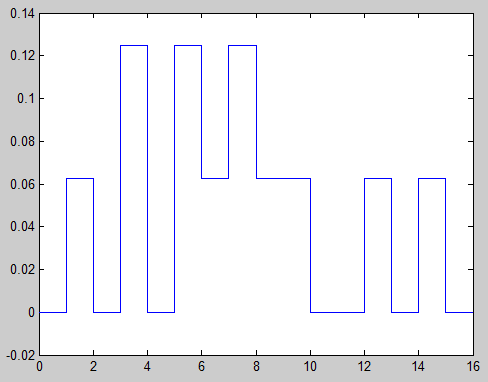
\includegraphics{./pictures/fft.png} \\ Рис.3 Результаты вычисления быстрой кросс-корреляции}
\\}

{\itemСравим время работы двух алгоритмов для случайных сигналов.
\flushright Таблица 1
\begin{center}
	\begin{tabular}{|p{3cm}|p{3cm}|p{3cm}|}
		\hline N&$t_{xcorr}$,c&$t_{fast}$,c \\
		\hline 20&0.00049&0.00014 \\
		\hline 50&0.00049&0.00014 \\
		\hline 100&0.00051&0.00013 \\
		\hline 200&0.00096&0.00018 \\
		\hline 500&0.0010&0.00022 \\
		\hline 1000&0.0012&0.00026 \\
		\hline 2000&0.0013&0.00034 \\
		\hline 5000&0.0023&0.00064\\
		\hline 10000&0.0042&0.0012 \\
		\hline 20000&0.0096&0.0023 \\
		\hline 50000&0.0669&0.0243 \\
		\hline 100000&0.0888&0.0308 \\
		\hline 
	\end{tabular}
\end{center}}

\section{Вывод}

Преобразование Фурье является математической основой спектрального анализа сигналов, который, в свою очередь, находит широкое применение в телекоммуникационных технологиях. Корреляционный анализ дает возможность установить в сигналах наличие связи. Например, для поиска известной последовательности во входном сигнале или неслучайных параметров в случайном сигнале.\\
В ходе работы мы сравнили работу двух алгоритмов для случайных сигналов. В итоге во всех тестовых примерах быстрая корреляция оказалась быстрее кросс-корреляции.

\end{enumerate}
\end{document}
